%--------------------------------------------------------------
%  Visualizing Recursion via JDI: Programmatic Breakpoints & Call Tree
%  A JDI-Based Debugger for Fibonacci (For CS Students)
%--------------------------------------------------------------
\documentclass[11pt,a4paper]{article}
\usepackage[utf8]{inputenc}
\usepackage[T1]{fontenc}
\usepackage{lmodern}
\usepackage{geometry}
\geometry{margin=1in}
\usepackage{listings}
\usepackage{xcolor}
\usepackage{graphicx}
\usepackage{caption}
\usepackage{hyperref}
\usepackage{float}
\usepackage{enumitem}
\usepackage{tikz}
\usetikzlibrary{arrows.meta, positioning, shapes}

%--- Code style --------------------------------------------------------
\lstset{
    language=Java,
    basicstyle=\ttfamily\small,
    keywordstyle=\color{blue}\bfseries,
    stringstyle=\color{red},
    commentstyle=\color{gray}\itshape,
    numbers=left,
    numberstyle=\tiny\color{gray},
    stepnumber=1,
    showstringspaces=false,
    tabsize=2,
    breaklines=true,
    frame=single,
    captionpos=b
}

\lstset{
    basicstyle=\ttfamily,
    columns=fullflexible
}

%--- Title ------------------------------------------------------------
\title{Visualizing Recursion with JDI:\\
Programmatic Breakpoints and Call Tree Construction}
\author{For Computer Science Students}
\date{\today}

\begin{document}
    \maketitle

    \begin{abstract}
        This article demonstrates how to **build a complete call tree** for a recursive method **without modifying its source code**.
        Using the **Java Debug Interface (JDI)**, we:
        \begin{itemize}
            \item Attach to a running JVM
            \item Set **programmatic breakpoints** on method entry/exit
            \item Read local variables and return values
            \item Reconstruct call hierarchy using **custom data structures**
        \end{itemize}
        The result: a **Graphviz tree** showing every call, its parameter, and return value.
    \end{abstract}

    \section{Target: Recursive Fibonacci}

    \begin{lstlisting}[caption={FibonacciTarget.java}]
public class FibonacciTarget {
    public static void main(String[] args) {
        int n = 5;
        long result = fibonacci(n);
        System.out.println("fibonacci(" + n + ") = " + result);
    }

    public static long fibonacci(int n) {
        if (n <= 1) return n;
        return fibonacci(n-1) + fibonacci(n-2);
    }
}
    \end{lstlisting}

    For \texttt{n=5}, there are **15 method invocations**.
    We want to **track each one**.

    \section{Approach: JDI + Programmatic Breakpoints}

    We use **JDI** to:
    \begin{enumerate}
        \item Start the target JVM in **debug mode** (JDWP)
        \item Attach a **remote debugger**
        \item **Programmatically** set:
        \begin{itemize}
            \item \texttt{MethodEntryRequest} — fires on method **entry**
            \item \texttt{MethodExitRequest} — fires on method **exit**
        \end{itemize}
    \end{enumerate}

    These act as **breakpoints**, but **without a GUI**.

    \begin{lstlisting}
MethodEntryRequest entry = eventManager.createMethodEntryRequest();
entry.addClassFilter("FibonacciTarget");
entry.enable();

MethodExitRequest exit = eventManager.createMethodExitRequest();
exit.addClassFilter("FibonacciTarget");
exit.enable();
    \end{lstlisting}

    \section{Core Data Structures}

    We build **three custom structures** to track calls:

    \subsection{\texttt{CallNode} — One Method Invocation}

    \begin{lstlisting}
private static class CallNode {
    final String id;           // Unique call ID (UUID)
    final int n;               // Input parameter
    final String parentId;     // Who called this?
    final List<CallNode> children = new ArrayList<>();
    long returnValue = -1;     // Result (set on exit)
}
    \end{lstlisting}

    \subsection{\texttt{callMap}: O(1) Lookup by ID}

    \begin{lstlisting}
private final Map<String, CallNode> callMap = new HashMap<>();
    \end{lstlisting}

    \begin{itemize}
        \item Key: \texttt{id} (UUID)
        \item Value: full \texttt{CallNode}
        \item Enables **fast access** on exit: \texttt{callMap.get(id)}
    \end{itemize}

    \subsection{\texttt{callStack}: Mirrors JVM Call Stack}

    \begin{lstlisting}
private final Deque<String> callStack = new ArrayDeque<>();
    \end{lstlisting}

    \begin{itemize}
        \item \texttt{push(id)} on **entry**
        \item \texttt{peek()} → **current parent**
        \item \texttt{pop()} on **exit**
        \item \textbf{LIFO} = exact JVM stack behavior
    \end{itemize}

    \begin{figure}[H]
        \centering
        \begin{tikzpicture}[
        box/.style={rectangle, draw, minimum width=2.5em, font=\small\ttfamily, align=center},
        arrow/.style={->, >=Stealth}
        ]
        \node[box] (s3) {id3};
        \node[box, below=of s3] (s2) {id2};
        \node[box, below=of s2] (s1) {id1};
        \node[below=of s1] {\small callStack};

        \draw[arrow, red] (s3) -- ++(2,0) node[right] {\texttt{peek()} → parent};
        \end{tikzpicture}
        \caption{\texttt{callStack} mirrors JVM stack → parent = top}
        \label{fig:stack}
    \end{figure}

    \section{Parent-Child via \texttt{callStack.peek()}}

    \begin{lstlisting}[caption={On Method Entry}]
String callId = UUID.randomUUID().toString();
String parentId = callStack.isEmpty() ? null : callStack.peek(); // KEY!
CallNode node = new CallNode(callId, n, parentId);
callMap.put(callId, node);
callStack.push(callId);

// Link to parent
if (parentId != null) {
    callMap.get(parentId).children.add(node);
}
    \end{lstlisting}

    \begin{itemize}
        \item \texttt{peek()} returns **who called the current method**
        \item This is **identical** to how the **JVM call stack** works
        \item No need to inspect stack frames — we **simulate** it
    \end{itemize}

    \begin{figure}[H]
        \centering
        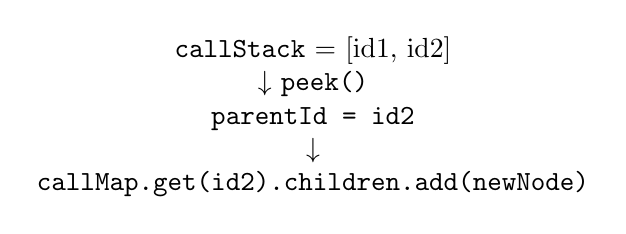
\begin{tikzpicture}
            \node[align=center] {
                \texttt{callStack} = [id1, id2] \\
                $\downarrow$ \texttt{peek()} \\
                \texttt{parentId = id2} \\
                $\downarrow$ \\
                \texttt{callMap.get(id2).children.add(newNode)}
            };
        \end{tikzpicture}
        \caption{Parent-child link built automatically}
    \end{figure}

    \section{Reading Parameters and Return Values}

    \begin{lstlisting}[caption={Reading local variable \texttt{n}}]
StackFrame frame = thread.frame(0);
for (LocalVariable var : frame.location().method().variables()) {
    if ("n".equals(var.name())) {
        n = ((PrimitiveValue) frame.getValue(var)).intValue();
    }
}
    \end{lstlisting}

    \begin{lstlisting}[caption={Capturing return value}]
if (event.returnValue() instanceof PrimitiveValue pv) {
    node.returnValue = pv.longValue();
}
    \end{lstlisting}

    Requires: \texttt{javac -g} (debug info)

    \section{Full Debugger Code}

    \lstinputlisting[caption={RecursionTreeDebugger.java}]{RecursionTreeDebugger.java}

    \section{Running the System}

    \begin{enumerate}
        \item Compile: \lstinline!javac -g FibonacciTarget.java!
        \item Start in debug mode:
        \lstinline!java -agentlib:jdwp=transport=dt_socket,server=y,suspend=y,address=*:5005 FibonacciTarget!
        \item Run debugger:
        \lstinline!java -cp .;<jdk>/lib/tools.jar;graphviz-java-*.jar;slf4j-*.jar RecursionTreeDebugger!
        \item Generate image:
        \lstinline!dot -Tpng fib_tree_debugger.dot -o fib_tree_debugger.png!
    \end{enumerate}

    \begin{figure}[H]
        \centering
        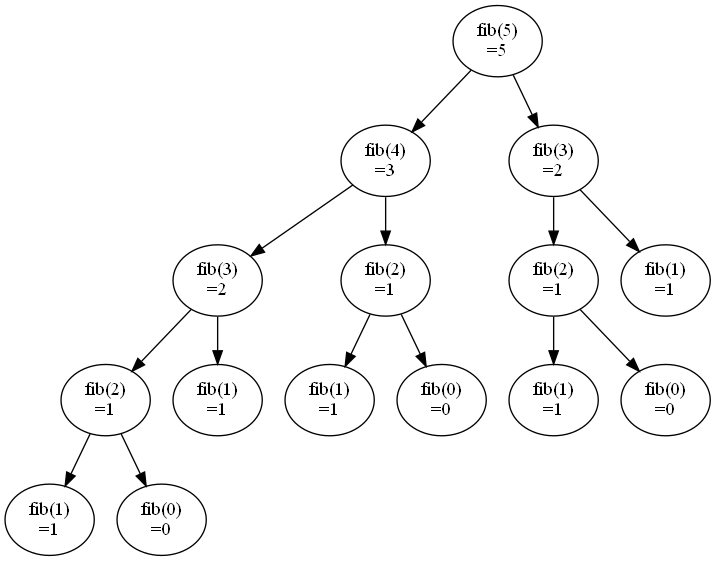
\includegraphics[width=0.9\linewidth]{fib_tree_debugger.png}
        \caption{Call tree: 15 nodes, correct hierarchy, return values}
        \label{fig:tree}
    \end{figure}

    \section{Key Insights}

    \begin{itemize}
        \item \textbf{No source changes} — works on any compiled class
        \item \textbf{Programmatic breakpoints} via JDI requests
        \item \textbf{\texttt{callStack} mirrors JVM} → correct parent tracking
        \item \textbf{\texttt{callMap} + UUIDs} → O(1) access, no collisions
        \item \textbf{Scalable} to deep or wide recursion
    \end{itemize}

    \section{Applications}

    \begin{itemize}
        \item Teaching recursion and call stacks
        \item Detecting redundant computation
        \item Visualizing algorithm behavior
        \item Extending to any recursive method
    \end{itemize}

    \section{Conclusion}

    By **attaching to the JVM**, **setting programmatic breakpoints**, and **mirroring the call stack** with \texttt{callStack}, we reconstruct the **full execution tree** of a recursive algorithm — **entirely at runtime**, **without instrumentation**.

    This is a powerful example of **JVM introspection** and **debugging automation**.

    \begin{table}[H]
        \centering
        \caption{Key Insights: JDI-Based Recursion Visualization}
        \label{tab:key-points}
        \begin{tabular}{|c|p{6.5cm}|p{6.5cm}|}
            \hline
            \textbf{No.} & \textbf{Key Point} & \textbf{Why It Matters} \\
            \hline
            1 & \textbf{JDI attaches to a running JVM} & No source code changes — pure runtime observation \\
            \hline
            2 & \textbf{Programmatic breakpoints via \texttt{MethodEntryRequest} / \texttt{MethodExitRequest}} & Breakpoints set in code, no IDE required \\
            \hline
            3 & \textbf{Read local variable \texttt{n} from stack frame} & \texttt{frame.getValue(var)} — requires \texttt{-g} debug info \\
            \hline
            4 & \textbf{Capture return value via \texttt{event.returnValue()}} & Direct access to result without logging \\
            \hline
            5 & \textbf{Unique \texttt{id} (UUID) per call} & Distinguishes identical \texttt{n} values \\
            \hline
            6 & \textbf{\texttt{callStack} (Deque<String>) mirrors JVM call stack} & LIFO ensures correct execution order \\
            \hline
            7 & \textbf{\texttt{peek()} → \texttt{parentId}} & Core mechanism for parent-child linking \\
            \hline
            8 & \textbf{\texttt{callMap} (HashMap<String, CallNode>) for O(1) lookup} & Fast node access on method exit \\
            \hline
            9 & \textbf{\texttt{CallNode} holds full call context} & Stores \texttt{id}, \texttt{n}, \texttt{parentId}, \texttt{children}, \texttt{returnValue} \\
            \hline
            10 & \textbf{Tree built automatically on entry} & \texttt{parent.children.add(child)} creates hierarchy \\
            \hline
            11 & \textbf{Output: \texttt{.dot} → Graphviz → PNG} & Fully automated visualization pipeline \\
            \hline
            12 & \textbf{100\% non-intrusive} & Works on any compiled class, any JVM \\
            \hline
        \end{tabular}
    \end{table}
\end{document}